
\section{Semi-Supervised ByteNet}

The ``Semi-Supervised Learning for NMT \ref{sec:theory:semi-supervised}'' theory section describes a general idea doing semi-supervised learning in neural machine translation. The method described does not depend on a specific machine learning architecture, but can in theory work using any supervised translation model.

The semi-supervised ByteNet model combines the generalized ``Semi-Supervised Learning for NMT'' ideas with the supervised ByteNet model.

\subsection{Synthetic Digits Problem}

The ByteNet model in itself is rather slow at learning, at least given the current state of TensorFlow. The strategy presented in ``Semi-Supervised Learning for NMT'' does not make this any better. In fact, because the unsupervised part of the loss requires inference using a beam search, the execution time will increase linearly with respect to the beam size. The situation may be even worse for ByteNet since ByteNet when used supervised allows for full parallelization over both the source and target sequence. When inference is done on the ByteNet model, as it is in the unsupervised case, only the encoder part is supervised.

Because of these complications, it is not feasible to apply the Semi-Supervised ByteNet model on the full Europarl v7 dataset and another monolingual (unlabeled) dataset. Instead, to show that the model works and validate the implementation, the model is applied to the synthetic digits problem.

Since the synthetic digits dataset can be randomly generated, 3 datasets created from 3 different random seeds are used. A bilingual (labeled) training dataset, a monolingual (unlabeled) training dataset, and a test dataset. The monolingual dataset does only contain the spelled out words. A fourth dataset containing only digits could also be used, but the original article showed that this had little benefit, thus to conserve computation time a fourth dataset was not used \cite{semi-supervised}.

The test dataset has 1024 observations, this includes most digits combinations. The number of observations in the bilingual and monolingual training dataset is varied in different experiments, to observe the effect of the dataset size.

The setup is identical to that in the purely supervised synthetic digits experiment, that was used to validate the ByteNet model. That is the dimensionality is set to 20, the Adam optimizer with a learning rate of 0.001 is used for optimization. The model ran for 300 epochs over the bilingual dataset. Additionally, the beam size for the unsupervised part is set to 5 sequences, and the model is parallelized over 2 GPUs.

This multi-GPU parallelization is done a little different that in the purely supervised experiments. Because the semi-supervised setup uses two separate translation models, the two translation models are kept on different GPUs. By doing this the weight updates doesn't have to be synchronized though the CPU, which does have some cost. The updates are however still done synchronously, there is just less I/O involved in the process.

\begin{figure}[h]
    \centering
    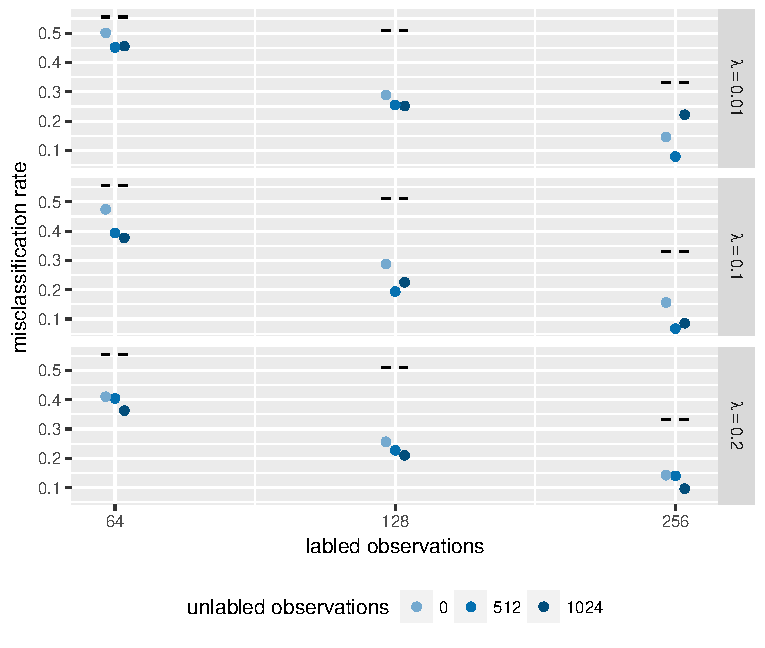
\includegraphics[scale=1]{semi-bytenet/synthetic-digits-grid.pdf}
    \caption{Shows the Semi-Supervised ByteNet model test performance depending on \textit{labeled dataset size}, \textit{unlabeled dataset size}, and \textit{unlabeled learning factor}.}
     \label{fig:result:semi-bytenet:missrate}
\end{figure}

\begin{figure}[h]
    \centering
    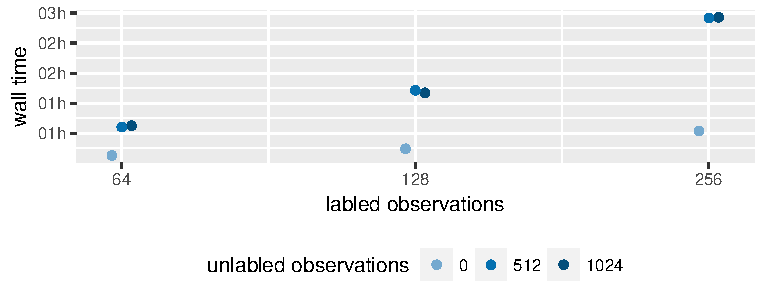
\includegraphics[scale=1]{semi-bytenet/synthetic-digits-grid-time.pdf}
    \caption{Shows the time spend running 300 epochs over the bilingual training dataset. The unlabeled learning rate is aggregated out (mean) since this has no theoretical nor practical performance impact.}
    \label{fig:result:semi-bytenet:time}
\end{figure}

In figure \ref{fig:result:semi-bytenet:time} the performance penalty for using unlabeled observations is very apparent. However, it is not as bad as one would theoretically expect. By using a beam size of 5 sequences, one would expect the training to run 5 times slower, but in practice, it is actually closer to 3. The computational performance is also independent of the unlabeled observations (as long as some are used), this is expected as the number of mini-batches used over 300 epochs only depends on the number of labeled observations.

The good performance can perhaps be explained by how well ByteNet parallelizes over the sequence length. While beam search does prevent this, a computational trick was used to allow some parallelization. By first performing the beam search on the ``text to digit'' translator and reapplying the ``text to digit'' translator (as well as the ``digits to text'' translator) the backward pass on the ``text to digit'' translator could be calculated in parallel. The forward and backward pass on the ``digits to text'' translator can also run in parallel, but this will also be the case for ByteNet. Another contributing factor to the performance is the small dimensionality of the ByteNet models used in the experiment, this likely means that the GPU has plenty of computational resources to run both the supervised and unsupervised part in parallel.

Figure \ref{fig:result:semi-bytenet:missrate} shows similar results to those in the original article, that article the research team found some improvement by using unlabeled observations, but nothing outstanding. This may sound like a disappointment, but in general, it is very hard to improve translation models dramatically. The fact that any translation model can likely be improved by using monolingual (unlabeled) data is actually very encouraging.

A significant difference between this experiment using the synthetic digits dataset and an experiment running on a proper natural language translation dataset is that the digits dataset has no variation in its output given the input. This means that ``one'' will always correspond to one, while in natural languages ``bitten'' in German can be understood as both a ``request'' and as an ''invite'' in English. This means that for a correct translation the unsupervised marginalization will approximately reduce to a marginalization over just one value, which is not very powerful. On the other hand for bad translations which is particularly common during the initial training, having a board beam in the beam search will definitely contribute to the model performance, though the multiple predicted translations in the marginalization. Indeed, if this was not the case it would be very hard to explain the performance improvements. \todo{Not super happy about this part.}

Finally, it is surprising that there is no difference between using 512 or 1024 unlabeled observations, or perhaps even a slight performance penalty for using 1024 unlabeled observations. A reasonable explanation is that using 512 observations covers the vast majority of the variation in the problem, adding the final 1024 observations thus doesn't add much. Furthermore, no insurance was made to prevent duplicate observations (observations was independently sampled). Given that there are only $10^3 + 10^2 = 1100$ different observations, it is very likely that many of the observation are duplicates, this is similar to the birthday probability paradox.
